\documentclass[runningheads]{llncs}
\usepackage{graphicx}
\usepackage{booktabs}
\usepackage{multicol}
\usepackage{tabularx}
\usepackage{float}
\restylefloat{table}


\begin{document}
%
\title{Data Mining 1: \\
Predicting positions of soccer players  \\
Project Report}
\authorrunning{Data Mining 1 Team 9}

\vspace{2cm}
\author{Team No. 9\\
\vspace{1cm}
presented by\\
Jurgen Amedani (1628022), Cara Maria Damm (1631263), Paul Hesselmann (1371380), Allwyn Menezes (1671634), Martin Mlinac (1364487), Carmen Rannefeld (1631070)\\
\vspace{1cm}
submitted to the \\
Data and Web Science Group\\
Prof. Dr. Bizer\\
University of Mannheim}

\institute{}
\maketitle
\newpage



%------------------------------------ Here goes out content
\section{Application Area and Goals}
\label{intro}
With soccer being the most popular sport worldwide it is not surprising that a good player is very expensive and that the soccer clubs are investing a lot of effort into the development of young talents \cite{ref_Transfermarkt}. One important aspect in the development of young talents is to identify the ideal position, so the player can exploit his full potential.
The question that arises is, are there specific attributes a goalkeeper, defender, midfielder and striker need to have? Is an ideal goalkeeper very tall and is it important that a defender has a stocky body type?\\
One way to evaluate if pattern exist is to analyze current soccer player and the position they are fulfilling. To do this we are using the FIFA 19 Dataset which is available on Kaggle.\\
FIFA 19 is a popular football simulation game based on the world class soccer player which was developed and released by Electronic Arts in September 2018. \\
The three main challenges for Data Scientists are collecting a significant amount of training data, cleaning and organizing the data as well as applying models  \cite{ref_Crowdflower}. Each challenge is time consuming which results into high cost.\\
In this paper we will evaluate different classification approaches, apply prepossessing methods an perform a comparison in terms of accuracy. For prepossessing the data, attributes were cleansed, some excluded and aggregated. A detailed description can be read in chapter \ref{sec:preprocessing}.
By applying different classification approaches an identification of the best approach to predict a players field position for unseen records is expected.

\section{Structure and Size of the Data}
In this project, which focuses on soccer analytics, the FIFA 19 dataset from Kaeggle is used. It includes information about every player who is registered to the SoFIFA database \cite{ref_sofifa}. 
The database includes more than 18207 registered players, for each player 86 different attributes are available. The attributes can be grouped in the following 10 groups: 
\begin{multicols}{2}
	\begin{enumerate}
	\item Personal information
	\item Contract Information
	\item Mental and Physical Capabilities
	\item Sports and Soccer Statistics
	\item Attacking Statistics  
	\item Skill Statistics
	\item Defending Statistics
	\item Movement Statistics
	\item Goalkeeping Statistics
	\item Strength Statistics
\end{enumerate}
\end{multicols}

Table 1 contains the attributes for each group:

\begin{table}[H]
\begin{tabular}{p{3.5cm}|p{8.5cm}l|l}
\hline 
Personal Information & Database ID,  Name, Age, Nationality, Height, Weight\\ 
\hline 
Contract Infromation &  Club, Wage, Release Clause, Jersey Number, Joined date, Loaned from, Contact valid until \\
\hline 
 Mental and Physical Capabilities & Agression, Interceptions, Positioning, Vision, Penalties, Composure\\
\hline
Sports and Soccer Information & Value, International Reputation, Overall Ranking, Potential (correlation to overall ranking), Special, Position (club), Position (national team), Preferred Foot, Week Foot, Skill Moves, Work Rate Defense, Work Rate, Attacking, Body Type,  Real Face \\
\hline
Attacking Statistics & Crossing, Finished, Heading Accuracy, Short Passing, Volleys \\
\hline
Skill Statistics & Dribbling, Curve, Free Kick Accuracy, Long Passing, Ball Control\\
\hline
Defending Statistics & Marking, Standing Tackle, Sliding Tackle\\
\hline
Movement Statistics & Acceleration, Sprint Speed, Agility, Reactions, Balance \\
\hline
Goalkeeping Statistics & GK Diving, GK Handling, GK Kicking, GK Positioning, GK Reflexes\\
\hline
Strength Statistics &  Shot Power, Jumping, Stamina, Strength, Long Shots\\
\hline
\end{tabular}
\label{tab:SelectionOfAttributes}
\caption{Selection of attributes}
\end{table}
In the data set one player is assigned to exactly one position out of 25 available positions. As players might play on different positions during a season or training, the potential for 24 positions (except goalkeeper position) is recognized as well in the data set. The position is written down as abbreviation meaning:
\begin{table}[H]
\begin{tabular}{p{3.5cm}|p{8.5cm}l|l}
\hline 
Forward& 	RF (Right forward), CF (Center forward), LF (Left forward),	RS (Right Striker),	ST (Striker), 	LS (Left Striker), RW (Right wing),	LW (Left wing) \\
\hline
Midfielder & 	LAM (Left attacking midfield), RAM (Right attacking midfield), CAM (Center attacking midfield), LM (Left midfield), CM (Central midfield), LCM (Left center midfield), (Right center midfield), RM (Right midfield),	LDM (Left defensive midfield), CDM (Center defensive midfield), RDM (Right defensive midfield)\\
\hline
Defensive & 
	LWB (Left Wing Back), RWB (Right Wing Back), LCB (Left center back), LB Left back), RCB (Right center back), CB (Center back), RB (Right back)\\
\hline
\end{tabular}
\label{tab:SelectionOfAttributes2}
\caption{Selection of attributes}
\end{table}
These position potentials are not applied for goalkeepers. 
Not all the attributes have filled values. One example is the \textit{loaned\_from} field which does not contain values for all the players since not every player is loaned from another club. Another reason for the missing information is that some players are young and not all the information has been collected yet. 
Analyzing the data set showed that there are 48 players were only key attributes like personal information are provided. \\
Attributes of the statistical groups are continuous data with a range from 0 to 100. Other attributes are categorical data. Furthermore the data set includes numerical attributes like wage, release clause, weight and height.
The wage and release clauses start with a value of 1000 while the specialty attribute is not smaller than 731.

\section{Preprocessing}
\label{sec:preprocessing}
Not all of the 86 attributes are needed to predict the position of a player therefore we applied the ``optimize selection operator'' and analyzed the log reports from Rapidminer to select the important attributes.
This showed that the following attributes:\textit{ sliding tackle, skill move, long passing, heading accuracy, finishing, crossing and sprint speed} were rated with a high relative importance. With no influence the other playing position results were weighted. More details and results of the attribute selection are described in the data mining chapter section \ref{sec:DM}.
%(Bild Einfügen)
Attributes marked as personal and contract information were excluded from the data set as they are not relevant to determine a players position. 
The data mining processes started with a higher aggregation of players position which were joined into four groups: \textit{defender, midfielder, striker and goalkeeper}. The following positions were grouped together into the attribute  \textit{Position\_grouped} replacing the original position attribute:

\begin{itemize} 
\item[] Striker:
\begin{itemize}
\item[-] ST, CF, LF, LS, LW, RF, RS, RW
\end{itemize}
\item[] Midfielder:
\begin{itemize}
\item[-] CAM, CDM, LCM, CM, LAM, LDM, LM, RAM, RCM, RD, RM
\end{itemize}
\item[] Defender:
\begin{itemize} 
\item[-] CB, LB, LCB, LWB, RB, RCB, RWB
\end{itemize}
\item[] Goalkeeper:
\begin{itemize}
\item[-] GK
\end{itemize}
\end{itemize}
After applying this aggregation 6838 midfielders, 2025 goalkeepers, 5866 defender and 3418 strikers (total 18147) are used to train the models. \textit{Position\_grouped }was marked as label in the classification model.\\
The attributes\textit{ release clause} and \textit{wage} are reported in a format including k (thousand) and m (million). These values have been converted. The \textit{height} is converted from foot into centimeter. The \textit{weight} has been recalculated from pound into kilogram. If there was no information provided for \textit{height} and \textit{weight} null values were added which allowed to exclude them by filtering. The attribute \textit{preferred foot }converted into a binomial value, meaning 0 for right and 1 for left. %The transformation of this attribute was not necessary as realized later.
Before the start of the training, examples were a value of \textit{position\_grouped} was missing were removed.\\
During the data mining process a second data set was prepared to test data and a potential overfit of the model. The test data set based on FIFA data from 2017 included 2652 midfielders, 632 goalkeeper, 2534 defenders and 1131 strikers (total 6949).
The FIFA17 data set was also extracted from the SoFIFA.com database two years ago. However, many of attribute names differ from FIFA19 data set which. Therefore  Rapidminer could not map the attributes directly and additional preprocessing steps were needed that included upper- and lower case renaming as well as changing abbreviations like "Free-kick accuracy" into "FKAccuracy".


\section{Data Mining}
\label{sec:DM}
To identify the best suited classification algorithm for our problem we applied K-Nearest Neighbors (KNN), Decision Trees, Gradient Boosted Trees, Deep Learning, Supported Vector Machines and Random Forest to the FIFA2019 data set.
Our mining process was separated in three phases: First, we ran the ''cross validation'' operator for each algorithm. Once we had first results for recall, precision and accuracy we transitioned in the second phase, where we aimed to optimize the results for each algorithm. Finally in the third phase we tested our learned models. To ensure that our models are neither under- nor overfitted we used the FIFA17 data set which varies from the FIFA19 data set.
In the following sections the different algorithms and their results from the first and second phase are presented.


\subsection{K-Nearest Neighbors (KNN)}
\label{sec:KNN}
K-Nearest Neighbors classifies unseen cases based on the k nearest neighbors. 
%As input to train our model FIFA 2019 data set is used. 
First, the ``optimize parameters" operator was applied for values of k between 1 and 100 as well as a 10-fold cross validation. The result of this optimization showed that the ideal value for k = 62 which provides an accuracy of 87.83\%. The best performing class was \textit{goalkeeper} with a precision of 100\% and the worst performing class was midfielder with a precision of 81.45\%. \\
Applying our model to the FIFA17 test data set the following results could be measured:\\
\begin{table}[H]
\label{Tab:knn}
\centering
\begin{tabular}{@{}lll@{}}
\toprule
                   & Training data & Test data \\ \midrule
Accuracy           & 87.83\%       & 87.37\%   \\
Weighted recall    & 88.46\%       & 87.92\%   \\
Weighted precision & 90.08\%       & 88.86\%   \\ \bottomrule
\end{tabular}
\caption{Results from KNN algorithm on training and test data}
\end{table}
In phase two of the mining process using KNN we started to optimize the algorithm by optimizing the attributes.
To do this we used the ``Optimize Selection'' and the ``Optimize Selection (Evolutionary)'' operator which determined the weight for the attributes based on the Gini Index and the Information Gain.
The optimal attributes are presented in table 4.
\begin{table}[H]
\begin{tabular}{p{3.5cm}|p{7.5cm}l|l}
\hline 
Optimize Selection (9) & Crossing, Finishing, HeadingAccuracy, ShortPassing, Dribbling, LongPassing, Vision, Marking, SlidingTackle\\
\hline
Information Gain (24)& Crossing, Finishing, HeadingAccuracy, ShortPassing, Volleys, Dribbling, FKAccuracy, LongPassing, BallControl, Acceleration, SprintSpeed, Agility, Balance, Jumping, Stamina, Strength, LongShots, Interceptions, Positioning, Composure, Marking, StandingTackle, SlidingTackle, Vision \\
\hline 
Gini Index (21) & Crossing, Finishing, HeadingAccuracy, ShortPassing, LongPassing, BallControl, Acceleration, SprintSpeed, Agility, Balance, Jumping, Stamina, Strength, LongShots, Interceptions, Positioning, Composure, Marking, StandingTackle, SlidingTackle, Vision\\ \hline
\end{tabular}
\label{Tab:knn2}
\caption{Selection of attributes}
\end{table}	
By selecting the attributes, the accuracy increased to 88.28 \% (Optimize Selection), 88.15 \% (Information Gain), 87.97\% (Gini Index). Table 5 shows the results on FIFA 2017 data set after the optimize selection.

\begin{table}[H]
\begin{tabular}{@{}llll@{}}
\toprule
                                        & Accuracy & Weighted Recall & Weighted Precision \\ \midrule
\multicolumn{1}{l|}{Optimize Selection} & 87.24\%  & 87.84\%         & 88.56\%            \\
\multicolumn{1}{l|}{Information Gain}          & 87.39\%  & 87.94\%         & 88.95\%            \\
\multicolumn{1}{l|}{Gini Index}         & 87.18\%  & 87.70\%         & 88.65\%            \\ \bottomrule
\end{tabular}
\label{Tab:KNNResults}
\caption{Results of KNN on test data}
\end{table}

As last optimization the ``Optimize Parameters" operator was used again, but only for the selected attributes with k values (1-100, 100 steps). This resulted to a k = 57 with the subset of attributes from the operator, and a k = 1 for both Information Gain and Gini Index. With this last optimization the test results couldn't be improved anymore and the accuracy dropped by 0.2\%.

\subsection{Result using Gradient Boosted Trees}

The gradient boosted trees algorithm is used to create an ensemble of decision trees trough gradually improved estimations. The output is a classification model which can be applied to the test dataset for a prediction of the label attribute position\_grouped. 
One advantage is the written report about the weights of attributes with respect to the label attribute.~\cite{ref_rapidminergbt}
The number of trees was set to 30. The maximal depth was initially set to 15, while the best result were scored with a maximal depth of 30.
The number of bins was set to 30.  
The process was executed with different settings regarding the maximal depth of trees. In summary, allowing a higher maximal depth resulted in better scores for $R^2$, recall and precision. Result of this values are shown in table \ref{Tab:GBT}.


\begin{table}[]
\begin{tabular}{@{}lllllll@{}}
\textbf{Run} & \textbf{\begin{tabular}[c]{@{}l@{}}Max. \\ tree depth\end{tabular}} & \textbf{\begin{tabular}[c]{@{}l@{}}Number \\ of folds\end{tabular}} & \textbf{Recall} & \textbf{Precision} & \textbf{$R^2$} & \textbf{\begin{tabular}[c]{@{}l@{}}Mean squarred\\ error\end{tabular}} \\
1            & 10                                                                  & 15                                                                   & 88,21 \%               & 89,01 \%                  & 64,4 \%                       & 0.33733332                                                             \\
2            & 15                                                                  & 15                                                                  & 88,05 \%               & 88,68 \%                  & 65,3 \%                       & 0.3289592                                                              \\
3            & 25                                                                  & 15                                                                  & 88,09 \%               & 88,70 \%                  & 65,4 \%                       & 0.3286427                                                              \\
4            & 30                                                                  & 15                                                                  & 88.09\%               & 88.73 \%                  & 65,4 \% & 0.328648                                                                     
\end{tabular}
\label{Tab:GBT}
\caption{Performance results of gradient boosted trees}
\end{table}

As important attributes the following were highlighted in table \ref{Tab:GBTImportantAttributes}:

\begin{table}[]
\begin{tabular}{@{}llll@{}}
\toprule
Variable        & \begin{tabular}[c]{@{}l@{}}Relative \\ Importance\end{tabular} & \begin{tabular}[c]{@{}l@{}}Scales \\ Importance\end{tabular}    & Percentage \\ \midrule
SlidingTackle   & 43887.371094        & 1.000000 & 0.179607   \\
Skill Moves     & 40664.996094        & 0.926576                      & 0.166419   \\
LongPassing     & 27751.718750        & 0.632340                      & 0.113572   \\
LCB             & 23368.140625        & 0.532457                      & 0.095633   \\
HeadingAccuracy & 22303.111328        & 0.508190                      & 0.091274   \\
LAM             & 16302.590820        & 0.371464                      & 0.066717   \\
Finishing       & 9715.319336         & 0.221369                      & 0.039759   \\
Crossing        & 9004.551758         & 0.205174                      & 0.036851   \\
SprintSpeed     & 5180.378906         & 0.118038                      & 0.021200   \\
ShortPassing    & 3899.299316         & 0.088848                      & 0.015958   \\ \bottomrule
\end{tabular}
\label{Tab:GBTImportantAttributes}
\caption{Important Attributes according to gradient boosted trees algorithm}
\end{table}
\subsection{Deep Learning}

Test Paul.\\

\subsection{Support Vector Machines}
Support Vector Machines (SVM) is a linear model for classification and regression problems. The SVM Linear takes a set of input data and predicts, for each given input, which of the two possible classes comprises the input, making the SVM a non-probabilistic binary linear classifier \cite{ref_rapidminersvm}.
We use cross validation for estimating statistical performance, classification by regression to build a polynomial classification model through regression learner and SVM linear to build a model that assigns new examples into one category or the other.\\
 A change in the value of the parameter C of SVM, which is the complexity constant, sets the tolerance for misclassification in its parameters where higher C values allow for `softer' boundaries and lower values create `harder' boundaries \cite{ref_rapidminersvm}.  A complexity constant that is large will lead to overfitting and values that are too small may result in over-generalization.\\
The algorithm looks at the extreme cases and draws a decision boundary known as hyperplane. The result from the optimization provides C for SVM Linear with the best value of 1.0. 
Training SVM on the FIFA 2019 data set, as shown in the table 7, leads to an the overall accuracy of 85.06\%. The best performing class is goalkeeper with 99.95\% accuracy and the worst performing class is strikers with 79.65\% accuracy. Precision and recall of the training set are 86.44\% and 87.87\% respectively. 
Applying the model to the test data set provides an overall accuracy of 83,74\% as shown in table 7. The best performing class is Goalkeeper with 100\% accuracy and the worst performing class is Striker with 76.10\% accuracy. The precision and recall of the test set obtained are 85.42\% and 85.76\% respectively. 

\begin{table}[]
\centering
\begin{tabular}{@{}l|ll@{}}
\hline
                    & Training & Testing \\ \hline
Accuracy            & 85,06 \% & \textbf{83,74\%} \\ \hline
Accuracy Goalkeeper & 99,95\%  & 100\%   \\
Accuracy Defender   & 87,1\%   & 87,9\%  \\
Accuracy Strikers   & 83,57\%  & 76,1\%  \\
Accuracy Midfielder & 79,65\%  & 79,04\% \\ \hline
Weighted Precision  & 86,44\%  & 85,42\% \\
Weighted Recall     & 87,87\%  & 85,76\% \\ \hline
\end{tabular}
\label{Tab:SVM}
\caption{Comparison of results of support vector machine algorithm}
\end{table}

\subsection{Random Forest}

At the end, we applied the random forest classifier as our sixth classification algorithm. In
general, Random Forests are used in classification and regression problems~\cite{ref_rapidminerRandomForest}.
A random forest is an ensemble method which consists of a collection of
multiple random decision trees. In many data sets, the Random Forest perform better than
decision tree classifiers ~\cite{ref_Tan}. Each tree is generated by random vectors of the training data sets. The nodes in the decision
trees are represented by the attributes. \newline 
When applying the model to new examples, each tree predicts a class by following the branches of the decision tree. The output is a voting
classification model which combines the decision trees in the random forest which means that
each tree in this forest make a decision and the class with the most votes determines the final
class. The classification of the random forest varies less than of each random tree on its own,
because every classification in the random forest is treated equally important. ~\cite{ref_rapidminerRandomForest} \newline
To find the optimal
values Optimize Parameter operator ran with different
values for number of trees (20 to 90 in steps of 7 with linear scale) and maximal depth (0 to
100 in steps of 10 with linear scale). Using the accuracy as splitting criterion. The resulting
optimal values for number of trees is 90 and for maximal depth is 50 (as well as: 76 for
number of trees and 100 for maximal depth and 90 for number of trees and 50 for maximal
depth). For the first combination of values, an accuracy of 88.39\% was scored, weighted precision of
90.22\% and a weighted recall of 89.15\%. Our best performing class was again the goalkeeper with a
precision of 100\% and our worst performing class was again the midfielder with a precision
of 83.53\%. The model was tested with FIFA17 data for the three
value combinations mentioned above. Different splitting criterions beside
Accuracy like Gain ratio, Information gain and Gini index were tried. The best result was archieved with
76 trees and a maximal depth of 100, using Information Gain as splitting criterion. The
results for this value combination are shown in table \ref{tab:RandomForest}.

\begin{table}[]
\begin{tabular}{@{}llll@{}}
\toprule
Splitting criterion                            & Accuracy         & Weighted Recall  & Weighted Precision \\ \midrule
\multicolumn{1}{l|}{Accuracy}                  & 84,63\%          & 85,77\%          & 87,13\%            \\
\multicolumn{1}{l|}{Gain Ratio}                & 87,55\%          & 87,67\%          & 89,24\%            \\
\multicolumn{1}{l|}{\textbf{Information Gain}} & \textbf{88,67\%} & \textbf{89,25\%} & \textbf{89,81\%}   \\
\multicolumn{1}{l|}{GINI index}                & 88,62\%          & 89,23\%          & 89,70\%            \\ \bottomrule
\end{tabular}
\label{tab:RandomForest}
\caption{Results of random forest model on test data}
\end{table}
\subsection{Evaluation setup and results}
\label{sec:Evaluation}
\subsection{Discussion of results}
\label{sec:DiscussionResults}
The perfect classification of goalkeepers can be justified by strength and weaknesses of these football positions.

 Goalkeepers have low values regarding sliding tackle, skill moves, sprint speed, etc. A visualization in a coordination systems \ref{fig:VisualAttributes} shows that goalkeepers (black) have the biggest deficits in these and other attributes (values in the bottom left corner). Defenders (blue) are better in these categories than goalkeepers. While midfielder (green) and strikers (orange) have nearly same strengths (one dot on top of each other in middle and top right corner). 

\begin{figure}
\centering
  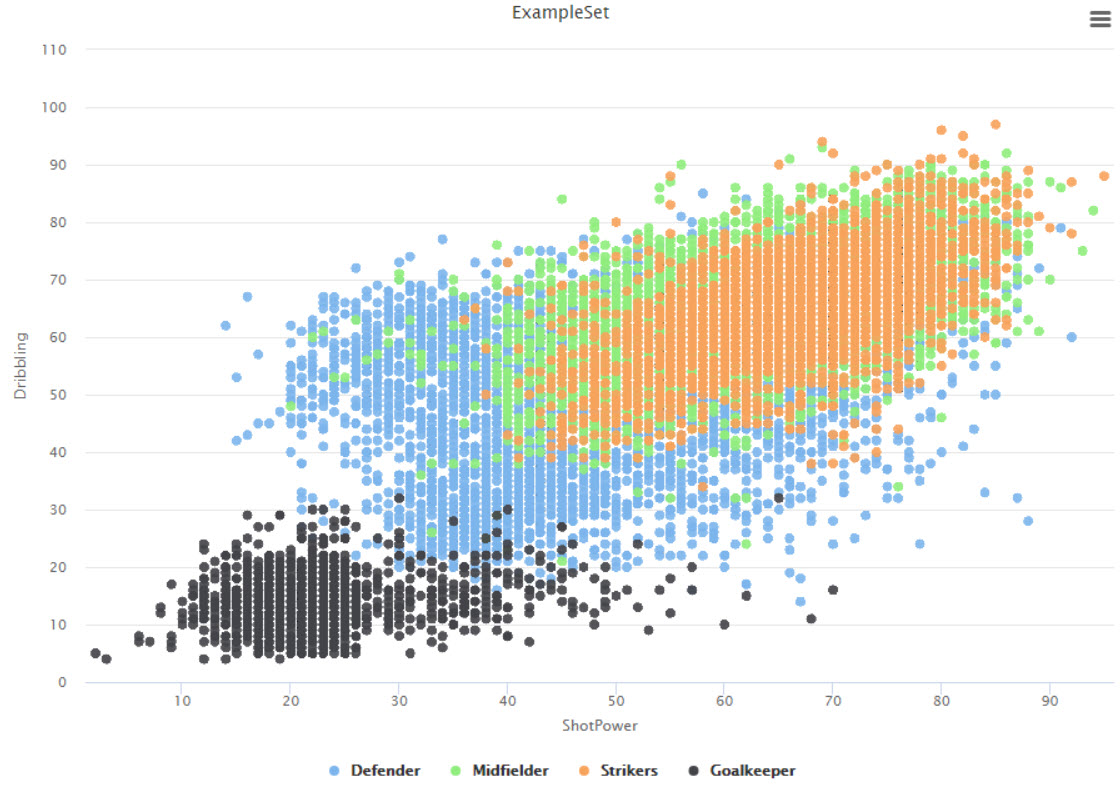
\includegraphics[width=8cm]{VisualizationAttributes.jpg}
  \caption{Visualization of two characteristics: dribbling and shot power}
  \label{fig:VisualAttributes}
\end{figure}

The result matches the expectations as the boundaries between strikers and midfielders are blurry. These two attributes are only an excerpt from more than 80 attributes but are typical for the data set.

As a conclusion, the data model to predict a soccer players position scores good result on the training and test data sets. Due to nearly identical attribute values for midfielders and strikers the accuracy decreased.




\newpage
% ---- Bibliography ----
%
% BibTeX users should specify bibliography style 'splncs04'.
% References will then be sorted and formatted in the correct style.
%

\bibliographystyle{splncs04}
\bibliography{mybibliography}
%
\begin{thebibliography}{8}

\bibitem{ref_Transfermarkt}
Die Transfermarkt Top Marktwerte, URL: \url{https://www.transfermarkt.de/1-bundesliga/marktwerte/wettbewerb/L1}. Last accessed May, 17 2019

\bibitem{ref_Crowdflower}
Crowdflower 2016 data science report, 2016   URL: \url{https://visit.figure-eight.com/data-science-report.html}. Last accessed May, 17 2019

\bibitem{ref_sofifa}
Sofifa.com \url{https://sofifa.com/players}. Last accessed May, 12 2019

\bibitem{ref_rapidminergbt}
Rapidminer Documentation GBT, URL: \url{https://docs.rapidminer.com/latest/studio/\newline operators/modeling/predictive/trees/gradient\_boosted\_trees.html}, last accessed May 12, 2019


\bibitem{ref_towardsGBT}
Towards Data Science: Understanding Gradient Boosting Machines, URL:  \url{https://towardsdatascience.com/understanding-gradient-boosting-machines-9be756fe76ab}. Last accessed May 22, 2019
%\bibitem{ref_gitplayerstatistics}
%Sofifa.com \url{https://github.com/amanthedorkknight/fifa18-all-player-statistics/blob/master/README.md}. Last accessed May, 12 2019

\bibitem{ref_rapidminerDeepLearning}
Rapidminer Documentation Deep Learning, URL: \url{https://docs.rapidminer.com/latest/\newline studio/operators/modeling/predictive/neural\_nets/deep\_learning.html}. Last accessed May 23, 2019

\bibitem{ref_rapidminersvm}
Rapidminer Documentation SVM, URL: \url{https://docs.rapidminer.com/8.2/studio/\newline operators/modeling/predictive/support\_vector\_machines/support\_vector\_machine.html}. Last accessed May 22, 2019

\bibitem{ref_rapidminersvm2}
Rapidminer Documentation SVM Evolutionary, URL: \url{https://docs.rapidminer.com/latest/studio/operators/modeling/predictive/\newline support\_vector\_machines/support\_vector\_machine\_evolutionary.html}. Last accessed May 22, 2019

\bibitem{ref_rapidminerRandomForest}
Rapidminer Documentation Random Forest, URL: \url{https://docs.rapidminer.com/latest/studio/operators/\newline modeling/predictive/trees/parallel\_random\_forest.html}. Last accessed May 22,2019

\bibitem{ref_Tan}
Tan, Pang-Ning, Michael Steinbach, and Vipin Kumar. Introduction to Data Mining. Pearson International ed. Boston Munich [u.a., 2006. Print. Pearson International Edition.]

\bibitem{ref_svm}
Rapid Miner Support Vector Machines, URL: \url{https://docs.rapidminer.com/8.2/studio/operators/modeling/predictive\newline/support\_vector\_machines/support\_vector\_machine.html}. Last accessed May 20, 2019
%
\bibitem{ref_svm2}
Rapid Miner Support Vector Machines Evolution, URL: \url{https://docs.rapidminer.com/latest/studio/operators/modeling/predictive\newline/support\_vector\_machines/support\_vector\_machine\_evolutionary.html}. Last accessed May 20, 2019

\bibitem{ref_towardsRFvsDecision}
Towardsdatascience.com, URL: \url{https://towardsdatascience.com/why-random-forests-outperform-decision-trees-1b0f175a0b5}. Last accessed May 23, 2019

\bibitem{ref_RFvsGBT}
Ravanshad,Abolfazl. Gradient Boosting vs Random Forest. URL: \url{https://medium.com/@aravanshad/gradient-boosting-versus-random-forest-cfa3fa8f0d80}. Last accessed May 23, 2019

\bibitem{ref_DL}
LeCun Y, Bengio Y, Hinton G. Deep learning. nature. 2015 May;521(7553):436.

\end{thebibliography}
\end{document}
